\documentclass[12pt]{article}
\usepackage[utf8]{inputenc}
\usepackage{float}
\usepackage{amsmath}


\usepackage[hmargin=3cm,vmargin=6.0cm]{geometry}
%\topmargin=0cm
\topmargin=-2cm
\addtolength{\textheight}{6.5cm}
\addtolength{\textwidth}{2.0cm}
%\setlength{\leftmargin}{-5cm}
\setlength{\oddsidemargin}{0.0cm}
\setlength{\evensidemargin}{0.0cm}

%misc libraries goes here
\usepackage{tikz}
\usetikzlibrary{automata,positioning}
\usepackage{amssymb}

\tikzstyle{block} = [rectangle, draw,text width=3.8em, text centered, minimum height=3.2em]

\begin{document}

\section*{Student Information } 
%Write your full name and id number between the colon and newline
%Put one empty space character after colon and before newline
Full Name : Hakan Bostan\\
Id Number : 2098812 \\

% Write your answers below the section tags
\section*{Answer 1}

\subsection*{a.}
Let $M=(Q,\Sigma ,\Gamma ,\delta ,q_0 , \Box ,F)$
$Q$ is the set of states.\\
$\Sigma = \{1,0\}$ is the input alphabet.\\
$\Gamma = \Sigma \cup \{<,>,\Box, \bullet,\vdash,\dashv\} \times \{0,1\}$\\
$\delta = (Q \times \Gamma) \rightarrow (Q \times \Gamma \times \{L,R\}$\\
$q_0$ is start state\\
$F$ is the set of final states.

On auxilary tape we hold the number of rows and number of columns in unary with a blank space between them. Second element of the tape characters holds the information of the heads coordinates. Only one element in the rows and one element in the columns has 1 as their second element.(e.g. if the 3rd 1 of the rows and the 2nd 1 of the columns has their second element as 1, that means ,back on 2d representation, the head is at (2,3) where 2 is column, 3 is row.). But on the main tape the second element of the tape characters represents whether the location is allocated or not (0 for unallocated, 1 for allocated). And also on the main tape we put a $\vdash$ representing the left end and $\dashv$ representing the right. After a ($\Box$,0) after $\vdash$ we start to list our rows. Rows are listed between $<$ and $>$ characters.\\

LA (Left Allocate): We find the 1 that has its second element as 1 in column section of the aux. tape and we change the tuple (1,1) to (1,0). Then we move main head and the aux head one to left. On aux tape if we see the tuple(1,0) we change it to (1,1), and on the main tape if we see ($<$,0) or ($\Box$,0) we shift all that is right of our current position to right and then we place ($\bullet$,1) on the current position. If we see the blank symbol between row number and column number we shift column numbers 1 place to right and we add a new 1 to the left of the column numbers. Also on the main tape (if our operations are correct we should see a $<$) we shift all that is right of our current position to right and then we place ($\bullet$,1) on the current position.If we see an already allocated cell (i.e (X,1)) we do nothing on the main tape.\\
\\
LB (Left Blank): We find the 1 that has its second element as 1 in column section of the aux. tape and we change the tuple (1,1) to (1,0). Then we move main head and the aux head one to left. On aux tape if we see the tuple(1,0) we change it to (1,1), and on the main tape if we see ($<$,0) or ($\Box$,0) we shift all that is right of our current position to right and then we place ($\Box$,1) on the position that has opened. If we see the blank symbol between row number and column number we shift column numbers 1 place to right and we add a new 1 to the left of the column numbers. Also on the main tape (if our operations are correct we should see a $<$) we shift all that is right of our current position to right and then we place ($\Box$,1) on the position that has opened.If we see an already allocated cell (i.e (X,1)) we do nothing on the main tape.\\
\\
RA (Right Allocate): We find the 1 that has its second element as 1 in column section of the aux. tape and we change the tuple (1,1) to (1,0). Then we move main head and the aux head one to right. On aux tape if we see the tuple(1,0) we change it to (1,1), and on the main tape if we see ($>$,0) or ($\Box$,0) we shift all that is right of our current position(this time including the $>$ symbol.) to right and then we place ($\bullet$,1) on the position that has opened. If we see the blank symbol on aux tape we place (1,1) on aux tape and do the same operations on the main tape.If we see an already allocated cell (i.e (X,1)) we do nothing on the main tape.\\
\\
RB (Right Blank): We find the 1 that has its second element as 1 in column section of the aux. tape and we change the tuple (1,1) to (1,0). Then we move main head and the aux head one to right. On aux tape if we see the tuple(1,0) we change it to (1,1), and on the main tape if we see ($>$,0) or ($\Box$,0) we shift all that is right of our current position(this time including the $>$ symbol.) to right and then we place ($\Box$,1) on the position that has opened. If we see the blank symbol on aux tape we place (1,1) on aux tape and do the same operations on the main tape.If we see an already allocated cell (i.e (X,1)) we do nothing on the main tape.\\
\\
UA (Up Allocate): We find the 1 that has its second element as 1 in row section of the aux. tape and we change the tuple(1,1) to (1,0). Then we move main head and the aux head one to left. On aux tape if we see $\vdash$ we shift everything on aux tape except $\vdash$ to right and write (1,1) to the opening. And on the main tape we move to the start (i.e. we go left till we see $\vdash$) after that we move everything on the main tape 4 places to the right (to create space for $<,\bullet,>$) then we place ($<$,0),($\bullet,1$),($>$,0),($\Box$,0). If we see (1,0) on aux tape when we move left, we write (1,1) instead and we do nothing on the main tape.\\
\\
UB (Up Blank) : We find the 1 that has its second element as 1 in row section of the aux. tape and we change the tuple(1,1) to (1,0). Then we move main head and the aux head one to left. On aux tape if we see $\vdash$ we shift everything on aux tape except $\vdash$ to right and write (1,1) to the opening. And on the main tape we move to the start (i.e. we go left till we see $\vdash$) after that we move everything on the main tape 4 places to the right (to create space for $<,\Box,>$) then we place ($<$,0),($\Box,1$),($>$,0),($\Box$,0). If we see (1,0) on aux tape when we move left, we write (1,1) instead and we do nothing on the main tape.\\
\\
DA (Down Allocate): We find the 1 that has its second element as 1 in the row section of the aux. tape nad we change the tuple(1,1) to (1,0). Then we move main head nad the aux head one to right. If we see a blank(which is between the row and column section) on aux tape, we shift everything on the aux tape to right creating space for an extra one in the row section of the tape. and we write (1,1) to the opening. And on the main tape we move to the right end and we just place ($<$,0),($\bullet$,1,0),{$>$,0),($\dashv$,0). If we see a (1,0) on the aux tape when we move right, we write (1,1) instead and we do nothing on the main tape.\\
\\
DB (Down Blank): We find the 1 that has its second element as 1 in the row section of the aux. tape nad we change the tuple(1,1) to (1,0). Then we move main head nad the aux head one to right. If we see a blank(which is between the row and column section) on aux tape, we shift everything on the aux tape to right creating space for an extra one in the row section of the tape. and we write (1,1) to the opening. And on the main tape we move to the right end and we just place ($<$,0),($\Box$,1,0),{$>$,0),($\dashv$,0). If we see a (1,0) on the aux tape when we move right, we write (1,1) instead and we do nothing on the main tape.\\
\\
T (Transpose access): We move to the start on the main tape, and to the start of the columns on the aux tape. We start moving right on the main tape and for every $<$ $>$ pair we see, we move one to the right on the aux tape and we stop when we see (1,1) tuple on aux tape, but we still move to the next $<$ on the main tape. Then we move to the beginning of the row section of the aux. tape.and we move the main head with aux. head. when we see a (1,1) we stop and check whether the main tape is allocated at that place. If it is not allocated, we return the main head back to its original place (just trace back the thing we have done so far). If it is allocated we transfer the row section of the aux tape to the end of the row section with a space in between. And we shift everything on the right of the beginning of the row section to left until we see $vdash$. We basically changed the row and column sections' places.\\

\subsection*{b.}
Actually I have used a semi-infinite tape in part a. Once I placed the $vdash$ symbol I have never moved it. I always expanded to the right thus simulating the semi-infinite tape. But for a two way infinite tape we can divide the tape at the head and we can say that one semi infinite tape holds whats left of the head and the other right of the head.
\subsection*{c.}
Yes it is equivalent, actually we thought of 2d machine as a n tape machine and we said that every tape represents a row. Since we can represent n tape machines with n-tuples on a single tape we were always actually working on a standard machine. Also we managed to turn our machine from 2d to 2-tape machine. And since we know that 2 tape machines are as powerful as standard machine M is also as powerful as standard machine.\\
\\
This function calculates $h(x)=log_5(2x)$.
\section*{Answer 2}

\subsection*{a.}
For this question I will employ two different machines to construct $M_f$.\\
First is a Divide-By-2 machine, which operates on a single tape and takes a unary input which is on the said tape. After calculating the half of the input it halts. During the process the input is lost.\\
$M_{Div2}=(Q,\Sigma ,\Gamma ,\delta ,q_0,\Box ,F)$\\
$Q=\{q_0 ,q_1 ,q_2 ,q_3 ,q_4 ,q_5 ,q_6,q_7\}$\\
$\Sigma= \{1,0 \}$\\
$\Gamma= \{1,0,\Box \}$\\
$\delta= (Q\times \Gamma)\rightarrow (Q\times \Gamma \times \{R,L,S\})$\\
$q_0$ is the initial state\\
$\Box$ is the blank symbol.\\
$Q_{accept}= \{q_7\}$\\
\\
Divide-By-2 machine:\\
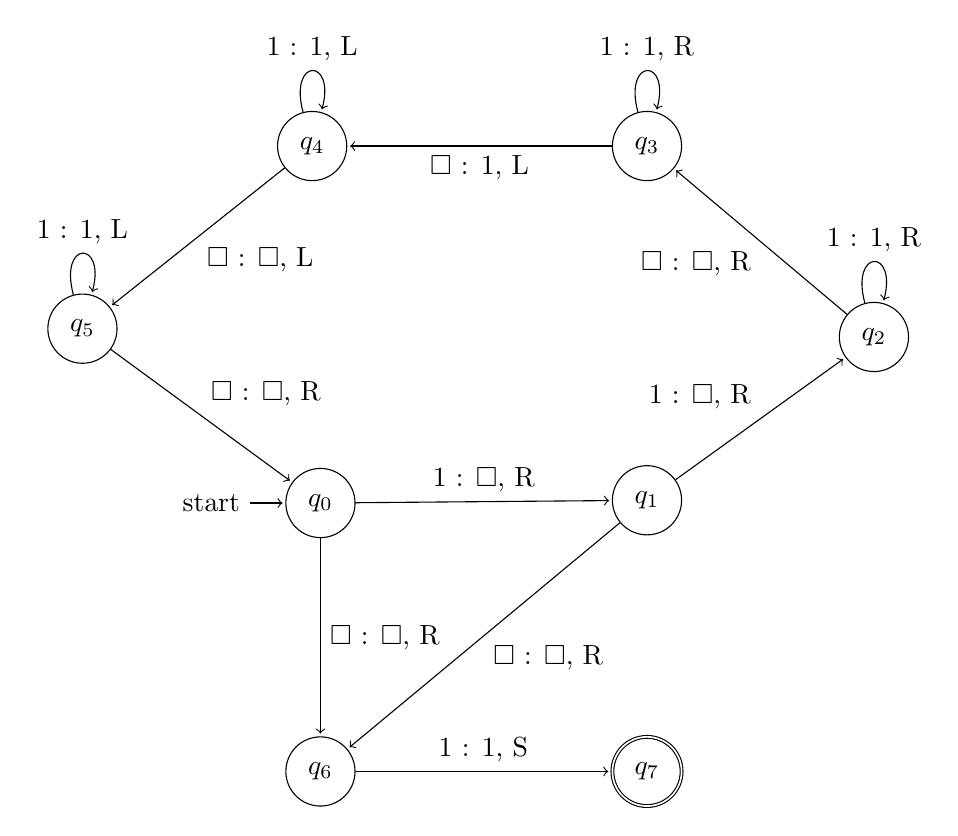
\begin{tikzpicture}[shorten >=1pt,node distance=1.5cm,on grid,auto]
  \draw (152.0pt, -153.0pt)node[state,initial](0){$q_{0}$};
  \draw (270.0pt, -152.0pt)node[state](1){$q_{1}$};
  \draw (352.0pt, -93.0pt)node[state](2){$q_{2}$};
  \draw (270.0pt, -24.0pt)node[state](3){$q_{3}$};
  \draw (149.0pt, -24.0pt)node[state](4){$q_{4}$};
  \draw (66.0pt, -90.0pt)node[state](5){$q_{5}$};
  \draw (152.0pt, -250.0pt)node[state](6){$q_{6}$};
  \draw (270.0pt, -250.0pt)node[state,accepting](7){$q_{7}$};
  \path[->] (1) edge node{1 : $\Box$, R}(2);
  \path[->] (1) edge node{$\Box$ : $\Box$, R}(6);
  \path[->] (4) edge node{$\Box$ : $\Box$, L}(5);
  \path[->] (6) edge node{1 : 1, S}(7);
  \path[->] (4) edge[loop above] node{1 : 1, L}(4);
  \path[->] (5) edge[loop above] node{1 : 1, L}(5);
  \path[->] (3) edge node{$\Box$ : 1, L}(4);
  \path[->] (0) edge node{$\Box$ : $\Box$, R}(6);
  \path[->] (2) edge[loop above] node{1 : 1, R}(2);
  \path[->] (3) edge[loop above] node{1 : 1, R}(3);
  \path[->] (2) edge node{$\Box$ : $\Box$, R}(3);
  \path[->] (5) edge node{$\Box$ : $\Box$, R}(0);
  \path[->] (0) edge node{1 : $\Box$, R}(1);
\end{tikzpicture}
\\
\\
Second is a comparator machine, which operates on two tapes and takes two separate inputs on two seperate tapes. If the input on the first tape(T1) is smaller than the second tape(T2) it writes 0 as output on T1, otherwise it writes 1 on T1.\\
$M_{Comp}=(Q,\Sigma ,\Gamma ,\delta ,q_0,\Box ,F)$\\
$Q=\{q_0 ,q_1 ,q_2\}$\\
$\Sigma= \{1,0 \}$\\
$\Gamma= \{1,0,\Box \}$\\
$\delta= (Q\times \Gamma^2)\rightarrow (Q\times \Gamma^2 \times \{R,L,S\})$\\
$q_0$ is the initial state\\
$\Box$ is the blank symbol.\\
$Q_{accept}= \{q_2\}$\\
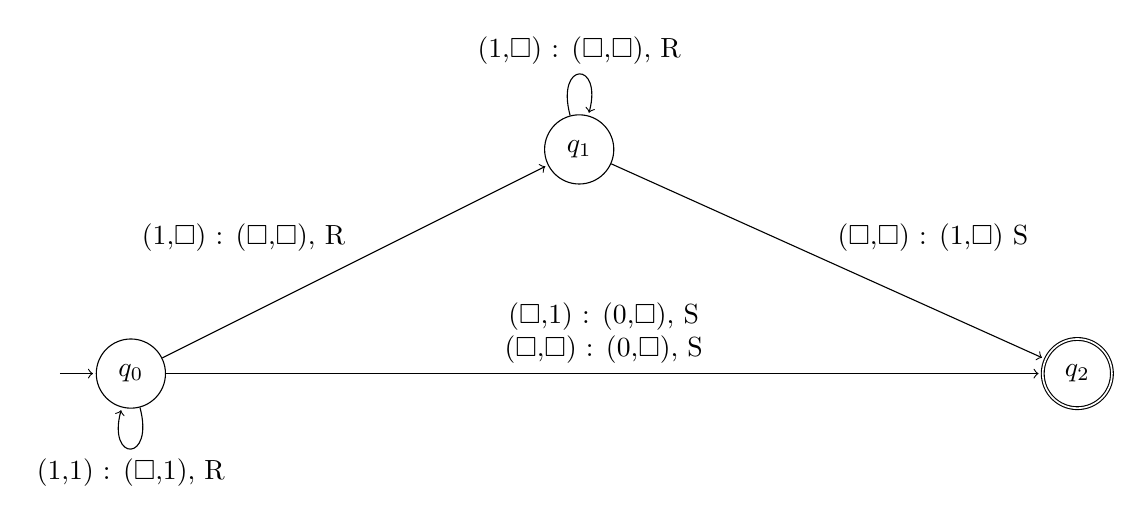
\begin{tikzpicture}[shorten >=1pt,node distance=1.5cm,on grid,auto]
  \draw (158.0pt, -221.0pt)node[state, initial, initial text =](0){$q_{0}$};
  \draw (320.0pt, -140.0pt)node[state](1){$q_{1}$};
  \draw (500.0pt, -221.0pt)node[state, accepting](2){$q_{2}$};
  \path[->] (0) edge node[align=center]{($\Box$,1) : (0,$\Box$), S\\ ($\Box$,$\Box$) : (0,$\Box$), S}(2);
  \path[->] (1) edge[loop above] node{(1,$\Box$) : ($\Box$,$\Box$), R}(1);
  \path[->] (0) edge[loop below] node{(1,1) : ($\Box$,1), R}(0);
  \path[->] (1) edge node{($\Box$,$\Box$) : (1,$\Box$) S}(2);
  \path[->] (0) edge node{(1,$\Box$) : ($\Box$,$\Box$), R}(1);
\end{tikzpicture}\\
\\
$M_f$ machine has two tapes with 2 seperate heads, and it takes two inputs on these tapes.\\
\\
$M_{f}=(Q,\Sigma ,\Gamma ,\delta ,q_0,\Box ,F)$\\
$Q=\{q_0 ,M_{Div2},M_{Comp},q_1\}$\\
$\Sigma= \{1,0 \}$\\
$\Gamma= \{1,0,\Box \}$\\
$\delta= (Q\times \Gamma^2)\rightarrow (Q\times \Gamma^2 \times \{R,L,S\}^2)$\\
$q_0$ is the initial state\\
$\Box$ is the blank symbol.\\
$Q_{accept}= \{q_2\}$\\
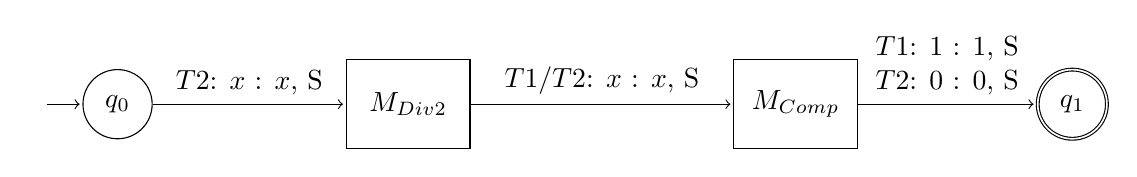
\begin{tikzpicture}[shorten >=1pt,node distance=1.5cm,on grid,auto]
  \draw (135.0pt, -234.0pt)node[state, initial, initial text =](0){$q_{0}$};
  \draw (240.0pt, -234.0pt)node[block](1){$M_{Div2}$};
  \draw (380.0pt, -234.0pt)node[block](2){$M_{Comp}$};
  \draw (480.0pt, -234.0pt)node[state, accepting](3){$q_{1}$};
  \path[->] (1) edge node{$T1/T2$: $x$ : $x$, S}(2);
  \path[->] (0) edge node{$T2$: $x$ : $x$, S}(1);
  \path[->] (2) edge node[align=center]{$T1$: 1 : 1, S \\ $T2$: 0 : 0, S}(3);
\end{tikzpicture}
\\ Here $M_{Div2}$ only operates on T2.
\subsection*{b.}
In construction of $M_g$ I will employ a new machine called $M_{Div5Rem}$ alongside $M{f}$ from part a.\\

$M_{Div5Rem}$ takes an input on a single tape and its output is the remainder and the quotient with a single blank between them.\\
\\
$M_{Div5Rem}=(Q,\Sigma ,\Gamma ,\delta ,q_0,\Box ,F)$\\
$Q=\{q_0 ,q_1 ,q_2 ,q_3 ,q_4 ,q_5 ,q_6,q_7,q_8,q_9,q_{10},q_{11},q_{12},q_{13}\}$\\
$\Sigma= \{1,0 \}$\\
$\Gamma= \{1,0,\Box \}$\\
$\delta= (Q\times \Gamma)\rightarrow (Q\times \Gamma \times \{R,L,S\})$\\
$q_0$ is the initial state\\
$\Box$ is the blank symbol.\\
$Q_{accept}= \{q_13\}$\\
\\
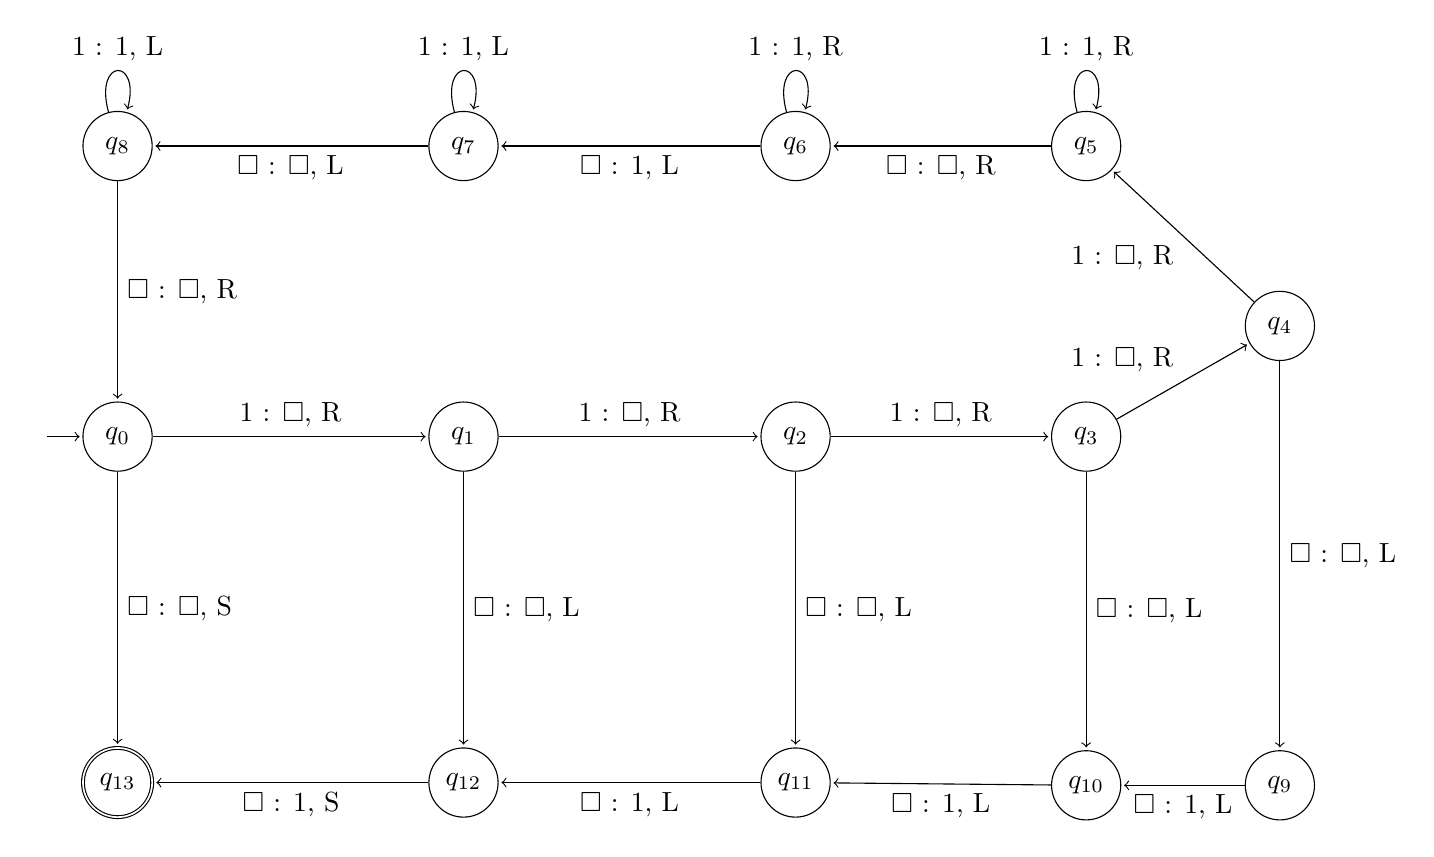
\begin{tikzpicture}[shorten >=1pt,node distance=1cm,on grid,auto]
  \draw (100.0pt, -180.0pt)node[state, initial, initial text =](0){$q_{0}$};
  \draw (225.0pt, -180.0pt)node[state](1){$q_{1}$};
  \draw (345.0pt, -180.0pt)node[state](2){$q_{2}$};
  \draw (450.0pt, -180.0pt)node[state](3){$q_{3}$};
  \draw (520.0pt, -140.0pt)node[state](4){$q_{4}$};
  \draw (450.0pt, -75.0pt)node[state](5){$q_{5}$};
  \draw (345.0pt, -75.0pt)node[state](6){$q_{6}$};
  \draw (225.0pt, -75.0pt)node[state](7){$q_{7}$};
  \draw (100.0pt, -75.0pt)node[state](8){$q_{8}$};
  \draw (520.0pt, -306.0pt)node[state](9){$q_{9}$};
  \draw (450.0pt, -306.0pt)node[state](10){$q_{10}$};
  \draw (345.0pt, -305.0pt)node[state](11){$q_{11}$};
  \draw (225.0pt, -305.0pt)node[state](12){$q_{12}$};
  \draw (100.0pt, -305.0pt)node[state, accepting](13){$q_{13}$};
  \path[->] (2) edge node{1 : $\Box$, R}(3);
  \path[->] (0) edge node{$\Box$ : $\Box$, S}(13);
  \path[->] (11) edge node{$\Box$ : 1, L}(12);
  \path[->] (12) edge node{$\Box$ : 1, S}(13);
  \path[->] (4) edge node{$\Box$ : $\Box$, L}(9);
  \path[->] (3) edge node{$\Box$ : $\Box$, L}(10);
  \path[->] (10) edge node{$\Box$ : 1, L}(11);
  \path[->] (7) edge node{$\Box$ : $\Box$, L}(8);
  \path[->] (7) edge[loop above] node{1 : 1, L}(7);
  \path[->] (8) edge[loop above] node{1 : 1, L}(8);
  \path[->] (6) edge node{$\Box$ : 1, L}(7);
  \path[->] (5) edge node{$\Box$ : $\Box$, R}(6);
  \path[->] (1) edge node{1 : $\Box$, R}(2);
  \path[->] (8) edge node{$\Box$ : $\Box$, R}(0);
  \path[->] (9) edge node{$\Box$ : 1, L}(10);
  \path[->] (1) edge node{$\Box$ : $\Box$, L}(12);
  \path[->] (5) edge[loop above] node{1 : 1, R}(5);
  \path[->] (6) edge[loop above] node{1 : 1, R}(6);
  \path[->] (3) edge node{1 : $\Box$, R}(4);
  \path[->] (0) edge node{1 : $\Box$, R}(1);
  \path[->] (4) edge node{1 : $\Box$, R}(5);
  \path[->] (2) edge node{$\Box$ : $\Box$, L}(11);
\end{tikzpicture}

$M_g$ has two tapes with separate heads, and it takes its input on its first tape(T1).\\
\\
$M_{g}=(Q,\Sigma ,\Gamma ,\delta ,q_0,\Box ,F)$\\
$Q=\{q_0 ,M_{Write5},M_{Div5Rem},M_{f},q_1\}$\\
$\Sigma= \{1,0 \}$\\
$\Gamma= \{1,0,\Box \}$\\
$\delta= (Q\times \Gamma^2)\rightarrow (Q\times \Gamma^2 \times \{R,L,S\}^2)$\\
$q_0$ is the initial state\\
$\Box$ is the blank symbol.\\
$Q_{accept}= \{q_1\}$\\
\\
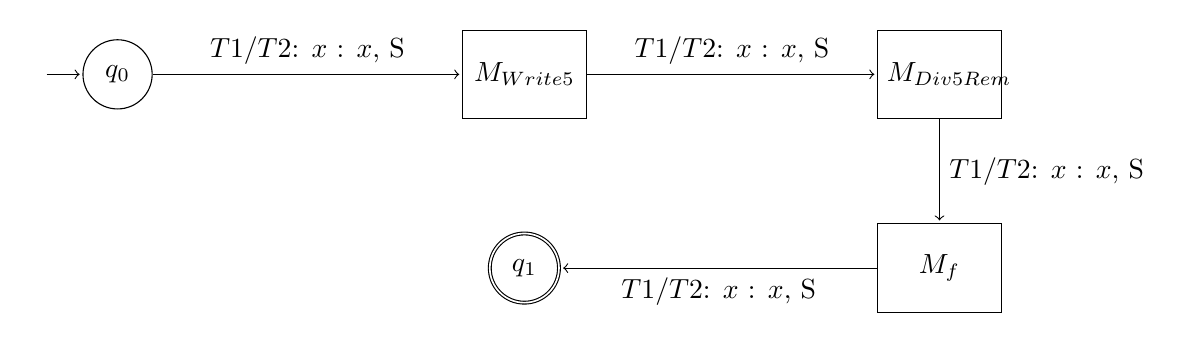
\begin{tikzpicture}[shorten >=1pt,node distance=1cm,on grid,auto]
  \draw (73 .0pt, -130.0pt)node[state, initial, initial text =](0){$q_{0}$};
  \draw (220.0pt, -130.0pt)node[block](1){$M_{Write 5}$};
  \draw (370.0pt, -130.0pt)node[block](2){$M_{Div5Rem}$};
  \draw (370.0pt, -200.0pt)node[block](3){$M_f$};
  \draw (220.0pt, -200.0pt)node[state, accepting](4){$q_{1}$};
  \path[->] (0) edge node{$T1/T2$: $x$ : $x$, S}(1);
  \path[->] (1) edge node{$T1/T2$: $x$ : $x$, S}(2);
  \path[->] (2) edge node{$T1/T2$: $x$ : $x$, S}(3);
  \path[->] (3) edge node{$T1/T2$: $x$ : $x$, S}(4);
\end{tikzpicture}
\\ Here $M_{Write5}$ only operates on T2 and writes unary 5 (i.e. 11111) on it.\\
$M_{Div5Rem}$ only operates on T1.\\
$M_{f}$ only operates on both T1 and T2.
\subsection*{c.}

$M_h$ has two tapes with separate heads and it takes input on first tape(T1) and gives it output on second tape(T2).\\
$M_{g}=(Q,\Sigma ,\Gamma ,\delta ,q_0,\Box ,F)$\\
$Q=\{q_0 ,M_{Write5},M_{Div5Rem},M_{f},q_1\}$\\
$\Sigma= \{1,0 \}$\\
$\Gamma= \{1,0,\Box,\triangleright\}$\\
$\delta= (Q\times \Gamma^2)\rightarrow (Q\times \Gamma^2 \times \{R,L,S\}^2)$\\
$q_0$ is the initial state\\
$\Box$ is the blank symbol.\\
$Q_{accept}= \{q_1\}$\\
\\
\begin{tikzpicture}[shorten >=1pt,node distance=1cm,on grid,auto]
  \draw (00.0pt, 0.0pt)node[state,initial, initial text=](0){$q_{0}$};
  \draw (100.0pt,0.0pt)node[state](1){$q_{1}$};
  \draw (210.0pt,0.0pt)node[block](2){$q_{g}$};
  \draw (350.0pt,0.0pt)node[state](3){$q_{3}$};
  \draw (350.0pt, 100.0pt)node[state](4){$q_{4}$};
  \draw (350.0pt, -100.0pt)node[state](5){$q_{5}$};
  \draw (450.0pt, -100.0pt)node[state](6){$q_{6}$};
  \draw (350.0pt, -200.0pt)node[state](7){$q_{7}$};
  \draw (210.0pt, -200.0pt)node[state,accepting](8){$q_{8}$};
  \path[->] (2) edge node{$T1/T2$: $x$ : $x$, S}(3);
  \path[->] (0) edge node{$T2$:$\Box$ : $\triangleright$, R}(1);
  \path[->] (1) edge node[align=center]{$T1/T2$:\\$x$ : $x$, S}(2);
  \path[->] (3) edge node[swap]{$T1$: 1 : 1, R}(5);
  \path[->] (5) edge node{$T2$: $\Box$: 1, S}(6);
  \path[->] (4) edge[swap, bend right] node{$T1$: 1 : 1, S}(1);
  \path[->] (5) edge[bend left] node[align=center]{$T1$: 1 : 1, L\\$T2$: $\Box$ : 1,R}(1);
  \path[->] (7) edge node{$T2$: $\triangleright$:$\triangleright$, R}(8);
  \path[->] (3) edge node{$T1$: 0 : $\Box$, R}(4);
  \path[->] (4) edge node[align=center]{$T1$: $\Box$:$\Box$, S \\ $T2$: $\Box$:$\Box$ ,L}(6);
  \path[->] (6) edge node{$T2$: 1:1, L}(7);
  \path[->] (7) edge[out=0,in=300,looseness=3] node{$T2$: 1:1, L}(7);
\end{tikzpicture}

\section*{Answer 3}

\subsection*{a.}

$M_f = (Q,\Sigma ,\Gamma ,\delta , q_0 , Q_{reject}, Q_{accept})$\\
$Q=\{q_0,q_1,q_2,q_{accept},q_{reject}\}$\\
$\Sigma = \{a,b,c \}$\\
$\Gamma = \{a,b,c,\Box \}$\\
$\delta = (Q \times \Gamma) \rightarrow (Q \times \Gamma \times \{R,L,S \} )$\\
$q_0$ is the initial state.\\
$Q_{reject} = \{ q_{reject}\}$\\
$Q_{accept} = \{ q_{accept}\}$\\

\begin{tikzpicture}[shorten >=1pt,node distance=1.5cm,on grid,auto]
  \draw (-4.0pt, 148.0pt)node[state, initial, initial text =](0){$q_{0}$};
  \draw (120.0pt, 149.0pt)node[state](1){$q_{1}$};
  \draw (-2.0pt, -29.0pt)node[state](2){$q_{2}$};
  \draw (218.0pt, -27.0pt)node[state, accepting](3){$q_{accept}$};
  \draw (388.0pt, -149.0pt)node[state, accepting](4){$q_{reject}$};
  \path[->] (0) edge[loop above] node{a : a, R}(0);
  \path[->] (1) edge[loop above] node{b : b, R}(1);
  \path[->] (2) edge[loop below] node{c : c, R}(2);
  \path[->] (0) edge node{b : b, R}(1);
  \path[->] (1) edge[swap] node{c : c, R}(2);
  \path[->] (0) edge[swap] node{c : c, R}(2);
  \path[->] (1) edge node{$\Box$ : $\Box$, S}(3);
  \path[->] (0) edge node{$\Box$ : $\Box$, S}(3);
  \path[->] (2) edge node{$\Box$ : $\Box$, S}(3);
  \path[->] (1) edge[out=0, in=90] node{a : a, R}(4);
  \path[->] (2) edge[bend right] node[align=center]{a : a, R\\ b : b, R}(4);
\end{tikzpicture}

\subsection*{b.}
Consider a TM with 3 tapes with seperate heads. At first we check the input with $M_f$ if $M_f$ halts on an accepting state we move the head to the beginning of the input. Then we check whether the input starts with an a. If so we skip 'a's untill we see a 'b'. When we see a 'b' we write 3 'a's on second tape for every 'a' that is currently on the second tape(e.g. if second tape has 3'a' s at a time, the next time we see a 'b' we write 3 'a's for the first 'a', 3 more for second 'a' and 3 more for the third 'a'. At the end, in total we have 9 'a's on the second tape). When we exhaust 'b's  on the first tape we return to the start of the input (which is on the first tape) and we compare 'a's one by one with the ones on the second tape. If the number of 'a's dont match we reject the input. If the number of 'a's match and we see a b on the first tape we append the contents of second tape to the third tape (which is initially empty). We do this append operation for every b on the first tape (thus multiplying the contents of the second tape $\textit{numberof 'b'}$ times and store it on the third tape.). At the end of the 'b's we compare the the number of 'c's in the first tape with the third tape, if it is an exact match we accept if not we reject.

\section*{Answer 4}

\subsection*{a.}
$L_2$ is finite, so we can create a finite automata for it which makes it regular.\\
$l_3$ is accepted by a DPDA so we can say that $L_3$ is DCFL.\\
$L_3 =\overline{L_1} \setminus L_2 =\overline{L_1} \cap \overline{L_2}$. Since $L_2$ is regular and since regular languages are closed under complementation $\overline{L_2}$ is also regular.We 
know that $L_3$ is DCFL and $\overline{L_2}$ is regular. If a language's intersection with a regular language results in a DCFL, that language should also be a DCFL. So from $L_3=\overline{L_1}
\cap \overline{L_2}$ we can conclude that $\overline{L_1}$ is a DCFL. And since DCFLs are closed under complementation $L_1$ is also a DCFL.\\
$L_4$ is recursively enumerable because a TM accepts the strings in $L_4$. $L_3$ is a DCFL, so it is also a recursively enumerable and since recursively languages are closed under concatanation
$L_3 L_4$ is a recursively enumerable language.\\
$L_5$ is a recursively enumerable language because there is a TM that can enumerate all the strings in $L_5$.\\
$\Sigma \cap \overline{L_3 L_4} = \overline{L_3 L_4}$ because $\Sigma $ denotes all strings. We have found that $L_3 L_4$ and $L_5$ are recursively enumerable. By Theorem 5.7.1 if $L_3 L_4$ is
recursively enumerable (which is true) then $L_3 L_4$ is recursive, because $\overline{L_3 L_4}=L_5$ and $L_5$ is recursively enumerable. $L_3$ is a DCFL so $L_3$ is also recursive. Recursive
languages are closed under concatanation so $L_4$ is recursive.\\

Also $L_5=\overline{L_3 L_4}$ and $\overline{L_5}=(L_3 L_4)$ so again by the Theorem 5.7.1 $L_5$ is recursive.\\
\\
Results:\\
$L_1$ is DCFL.\\
$L_2$ is Regular.\\
$L_3$ is DCFL.\\
$L_4$ is Recursive.\\
$L_5$ is Recursive.
 
\subsection*{b.}
$L_3$ is a DCFL so it has a DPDA. DCFLs are closed under compelement so $\overline{L_3}$ also has a DPDA. We can transform this DPDA to into a TM which accepts when an input is in $\overline{L_3}$ and rejects when an input is not in $\overline{L_3}$.(A deciding TM X)\\
$L_5$ is a recursive language, recursive languages are closed under reversal so $L_5^R$ is also recursive. That means we can construct a TM that decides whether a string is in $L_5^R$ or not.(A deciding TM Y)\\

Then we work X and Y in together if one of them halts in an accepting state(even if the other ends up in a rejecting state) we accept the input (i.e. input is in the language $L_5^R \cup \overline{L_3}$). We reject the input only when two of the machines end up in a rejecting state.And since we can create a deciding TM for $L_5^R \cup \overline{L_3}$, we can say that $L_5^R \cup \overline{L_3}$ is a Recursive language.\\

\end{document}

​

